\chapter{Os modelos constitutivos} \label{Cap: ModConst}

Em eventos onde deformações inelásticas estão presentes as tensões são modeladas de forma decomposta. De acordo com \cite{Holzapfel} todo tensor pode ser decomposto de forma aditiva em uma parcela esférica e uma desviadora. No caso dos tensores de tensão, a parcela esférica é oriunda de deformações que alteram o volume e a desviadora advém de deformações isocóricas. A decomposição aditiva do tensor de tensões de Cauchy é apresentada a seguir

\begin{equation} 
    \boldsymbol{\sigma} = \boldsymbol{s} - p\boldsymbol{I}
\end{equation}

Nela $ \gls{I} $ é o tensor identidade, $\boldsymbol{s}d$ é a parcela desviadora das tensões e $p$ é a pressão. Em eventos onde há presença de ondas de choque, a parte isocórica do tensor de tensões é modelada por uma equação constitutiva e a parte esférica por uma equação de estado. Antes de apresentar os modelos constitutivos mais usados é importante visitar alguns pontos da teoria da plasticidade, já que ela terá grande importância na definição do comportamento dos materiais quando submetidos à cargas elevadas. \\

De acordo com \cite{hiermaier_2008} a deformação irreversível de materiais é resultado de alterações na sua microestrutura. Destacam-se o movimento de discordâncias, o crescimento e o coalescimento de micro vazios como mecanismos citados por \cite{hiermaier_2008}. Estas alterações microestruturais são causadas por solicitações que elevam o material a tensões superiores à de resistência ao escoamento. De acordo com \cite{tadmor_miller_elliott_2012} a mecânica do contínuo não toma conhecimento da estrutura do material para descrever seu comportamento. Tal consideração faz com que fenômenos de ordem microestrutural não sejam levados em consideração direta, no entanto eles são considerados de forma indireta por meio de variáveis de estado internas, usadas nos modelos constitutivos. \\

De acordo com \cite{Holzapfel} as variáveis internas não podem ser mensuradas em um ensaio, porém são usadas para descrever o estado do material. O comportamento mecânico do material é associado ao seu estado, por exemplo: A tensão é calculada em função das variáveis de estado, por meio da relação constitutiva. Um exemplo de variável interna, que pode ser usada para descrever o estado e por conseguinte o comportamento do material, é o dano. Ele é calculado por vários modelos e em alguns deles é usado para definir a resistência do material, porém não há como medi-lo diretamente em um laboratório. \\

 A avaliação do comportamento esperado para o material deve considerar os pormenores de seu estado para saber se as alterações no ambiente ou no tipo de solicitação fazem com que haja mudança nas propriedades previamente observadas. De acordo com \cite{Zukas} dados obtidos em condições de baixa pressão e em situações quasi-estáticas dificilmente serão uteis para a simulação de um evento em alta velocidade. \par

As propriedades dos materiais podem apresentar grandes diferenças quando diferentes taxas de deformação são aplicadas. No extremo inferior da taxa de deformação a fadiga pode estar presente caso as condições de temperatura e carga sejam propicias. No extremo superior, a solicitação de materiais devido à explosões faz com que a resistência do material possa ser completamente ignorada, quando estes eventos são simulados. Este trabalho busca apresentar os modelos constitutivos inseridos no contexto de impactos de media velocidade. Por média velocidade entende-se que os impactos não levam o material ao estado de choque. De acordo com \cite{Zukas} este tipo de impacto são são aqueles onde a velocidade do projetil não supera os $2000 m/s$. De acordo com \cite{Hazell} a velocidade limítrofe para o inicio da observação de ondas de choque depende do material impactado, elas surgem quando a velocidade de penetração supera a velocidade do som no meio. \par


Quando não há presença de ondas de choque, o material pode ser modelado apenas por uma relação constitutiva ou por uma relação constitutiva e uma equação de estado, além disso equações de estado muito mais simples podem ser usadas neste tipo de situação. De acordo com \cite{hiermaier_2008} a plasticidade computacional oferece base teórica para os modelos constitutivos usados na balística. \\

\section{Plasticidade perfeita, isotrópica e cinemática.}

De acordo com \cite{neto_peric_owens_2008} quando um corpo se deforma plasticamente ele pode apresentar, um ou uma mistura destes três tipos de plasticidade. 
\begin{itemize}
    \item Plasticidade perfeita.
    \item Plasticidade Isotrópica
    \item Plasticidade cinemática.
\end{itemize}
\par

A plasticidade perfeita é caracterizada pela estabilidade da tensão de escoamento. Nela o material escoa sem aumentar a resistência a futuras deformações plásticas. Uma curva de carga e descarga que apresenta plasticidade perfeita pode ser vista na figura \ref{fig:plastperf}. Não há alteração da tensão de escoamento, tal comportamento independe da quantidade de deformação que o material sofre. \\ 
\begin{figure}[H]
    \centering
    \caption{Curva de tensão deformação apresentando plasticidade perfeita. }
    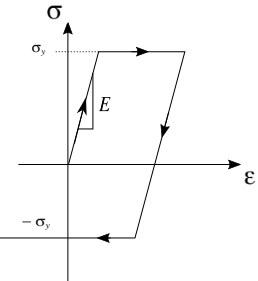
\includegraphics[width=0.5\linewidth]{images/plasticidade_perfeita.png}
    \label{fig:plastperf}
    \fonte{O autor (2020)}
\end{figure}

O segundo comportamento típico é a plasticidade isotrópica. Nela a tensão limite de escoamento é alterada por conta de deformações plásticas. Portanto, caso uma tensão trativa gerar deformação plástica em um ponto, um subsequente ciclo de carregamento necessitará de maior tensão trativa para gerar deformação plástica neste mesmo ponto. O característico da plasticidade isotrópica é que o aumento do limite de escoamento em tração significa também um aumento do limite de escoamento em compressão.
Portanto, como mostra a figura \ref{fig:plastiso}, um ciclo de carregamento em tração gera deformação plástica, aumentando o limite de escoamento tanto em tração quanto em compressão. Um ciclo subsequente em compressão precisará atingir a tensão de escoamento inicial $\sigma_y$ somada a um delta de tensão $d\sigma$ para provocar deformação plástica. 

\begin{figure}[H]
    \centering
    \caption{Curva de tensão deformação apresentando plasticidade isotrópica. }
    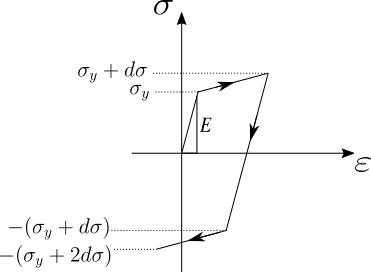
\includegraphics[width=0.5\linewidth]{images/plasticidade_iso.png}
    \label{fig:plastiso}
    \fonte{O autor (2020)}
\end{figure}

O último modo de plasticidade é a cinemática, nela a tensão limite de escoamento também é alterada de acordo com o nível de deformação plástica do material. Entretanto, a distância entre a tensão limite de escoamento em tração e em compressão se mantém igual ao longo do tempo. Portanto, um acréscimo na resistência à tensão trativa significa um decréscimo correspondente na resistência à tensão compressiva, vide figura \ref{fig:plastcin}.  \par

\begin{figure}[H]
    \centering
    \caption{Curva de tensão deformação apresentando plasticidade cinemática. }
    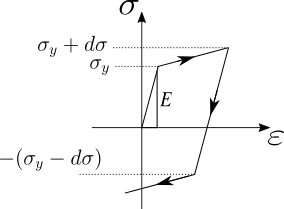
\includegraphics[width=0.5\linewidth]{images/plasticidade_cinem.png}
    \label{fig:plastcin}
    \fonte{O autor (2020)}
\end{figure}

Nos casos onde há alteração da tensão de escoamento, por conta da deformação plástica, é possível o endurecimento ou encruamento ocorra de forma linear ou não linear. A figura \ref{fig:plastlinvsnlin} exemplifica a diferença entre a plasticidade isotrópica linear e não linear. \par

\begin{figure}[H]
    \centering
    \caption{Comparação de encruamento linear versus não linear. } 
    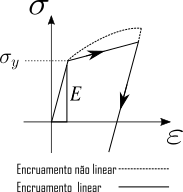
\includegraphics[width=0.8\linewidth]{images/plasticidade_linnlin.png}
    \label{fig:plastlinvsnlin}
    \fonte{O autor (2020)}
\end{figure}

Nada impede que estes comportamentos ocorram ao mesmo tempo. Portanto, um material pode, por exemplo, se comportar de forma isotrópica cinemática não linear. \\

\section{A superfície de escoamento e o espaço das tensões principais}

Até agora a tensão foi tratada como sendo escalar, portanto tratava-se da tensão observada em um estado uniaxial de tensão. \footnote{Aqui existe a repetição da palavra tensão pois o estado uniaxial de deformação existe e é importante no campo da balística.} O campo de tensões reais é descrito por um tensor, $ \gls{Cauchy} $, que contém nove componentes, sendo seis delas independentes entre si. O limite de escoamento, outrora escalar, agora é uma hiper superfície em seis dimensões. A descrição de um espaço hexa dimensional não é trivial, por conta disso, de acordo com \cite{hiermaier_2008},  foi criada uma descrição que usa a decomposição espectral do tensor de tensões.\footnote{O teorema responsável por tal decomposição é o teorema 
espectral e pode ser encontrado em \cite{gurtin_fried_anand_2013} pg. 28. } \\

O espaço característico do tensor de tensões é composto por seus auto vetores e auto valores. O teorema espectral torna possível escrever o tensor usando três componentes, que são posicionados na diagonal da matriz que representa o tensor. 
No contexto do tensor de tensões de Cauchy decomposto de forma espectral. Os auto valores são chamados de tensões principais e são os valores das componentes. Os auto vetores são representados pela linha da na matriz e são chamados de direções principais. Em forma matricial o tensor de tensões de Cauchy, descrito de forma espectral, é apresentado a seguir.

\begin{equation}
\gls{Cauchy} = 
    \begin{bmatrix}
    \sigma_1 & 0 & 0 \\
    0 & \sigma_2 & 0 \\
    0 & 0 & \sigma_3
    \end{bmatrix}
\end{equation}

Como dito anteriormente, é costumeiro decompor de forma aditiva o tensor de tensões. Esta decomposição é feita em duas parcelas, uma desviadora e a outra volumétrica. Portanto, apresenta-se a parcela desviadora do tensor de tensões quando decomposto de forma espectral.

\begin{equation}
\boldsymbol{S} = 
    \begin{bmatrix}
    S_1 & 0 & 0 \\
    0 & S_2 & 0 \\
    0 & 0 & S_3
    \end{bmatrix} = \begin{bmatrix}
    \sigma_1 - \sigma_m & 0 & 0 \\
    0 & \sigma_2 - \sigma_m & 0 \\
    0 & 0 & \sigma_3 - \sigma_m
    \end{bmatrix}
\end{equation}

Onde 
\begin{equation}
     \sigma_m = \frac{\sigma_1 + \sigma_2 + \sigma_3}{3}
\end{equation}

No espaço característico do tensor de Cauchy, a superfície de escoamento anteriormente em seis dimensões torna-se uma superfície em três dimensões, que pode ser descrita e entendida de forma mais simples. De acordo com \cite{hiermaier_2008} o espaço das tensões principais chama-se Espaço de Haigh-Westergaard, em referência aos pesquisadores que sugeriram tal descrição. Neste espaço o estado de tensões hidrostáticas é representado pela eq. \ref{eq:hydrostress}, onde $ J_1 $ é o primeiro invariante do tensor de tensões desviadoras. Neste estado as tensões desviadores $S_i$ são nulas, portanto a diagonal formada pela eq. \ref{eq:hydrostress} é chamada de eixo hidrostático.  

\begin{equation} \label{eq:hydrostress}
    \sigma_1 = \sigma_2 = \sigma_3 = \frac{1}{3} J_1
\end{equation}

Os invariantes $\gls{prinvadesv}$ das tensões desviadoras são usados para definir critérios de escoamento. Eles são aplicados nas funções que descrevem a superfície de escoamento. Existem algumas coordenadas que possuem leitura mais clara no espaço de haigh-Westergaard, que por sua vez são chamadas de coordenadas de Haigh-Westergaard. A descrição gráfica destas coordenadas é mostrada na figura \ref{fig:coordhaigh}. Uma explicação das coordenadas será dada a seguir, porém para tal é necessário definir o que são planos desviadores e meridianos. Planos desviadores são aqueles cuja normal é o eixo hidrostático, mover-se por um plano desviador significa alterar o estado de tensões desviadoras. Meridianos são perpendiculares aos planos desviadores e contém o eixo hidrostático, mover-se ao longo de um meridiano significa mudar o estado de tensão hidrostática mantendo constante a coordenada $\theta$. A figura \ref{fig:coordhaigh} apresenta tanto um plano desviador quanto um meridiano. \\

\begin{itemize}
    \item $ \xi $: Tem relação direta com o estado de pressão do material, portanto acompanha o eixo hidrostático.
    \item $ \rho $: Medida da distância do eixo hidrostático até a superfície de escoamento em um plano desviador.
    \item $ \theta $: Refere-se à triaxialidade das tensões, de acordo com \cite{hiermaier_2008}.
    \begin{itemize}
        \item $\theta \, = \, 0 º$: Estado hidrostático sobreposto por tração uniaxial.\footnote{Os estados hidrostáticos dependem apenas da coordenada $\xi$}
        \item $\theta \, = \, 30 º$: Estado hidrostático sobreposto por cisalhamento puro.
        \item $\theta \, = \, 60 º$: Estado hidrostático sobreposto por compressão uniaxial. 
    \end{itemize}
\end{itemize}


\begin{figure}[H]
    \centering
    \caption{Coordenadas de Haigh-Westergaard traduzida de \cite{hiermaier_2008}}
    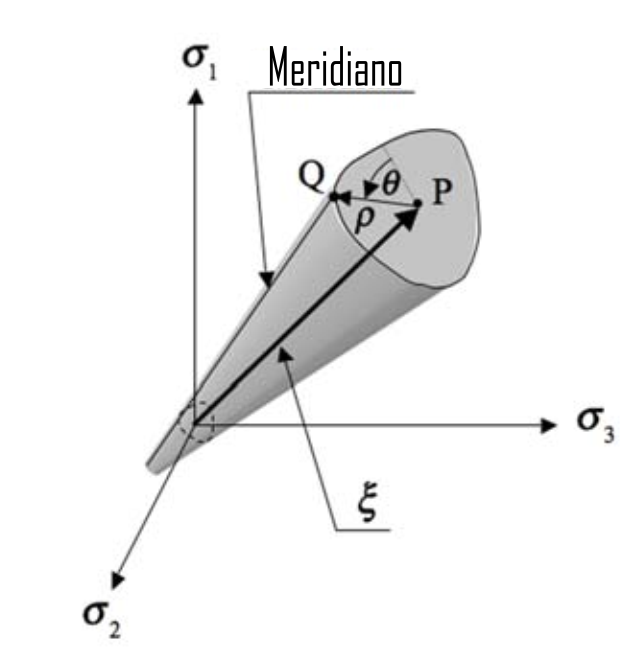
\includegraphics[width=0.5\linewidth]{images/Haigh_Wester.png}
    \label{fig:coordhaigh}
    \fonte{O autor (2020)}
\end{figure}

\section{O critério de escoamento}

O critério de escoamento pode ser representado através de uma função que pode ter como variáveis independentes os invariantes do tensor de tensões desviadoras, as coordenadas de haigh-Westergaard, os invariantes do tensor de tensões ou as tensões principais. \\

\subsection{Escoamento independente da pressão.}

 \cite{hill} mostrou que não há dependência da pressão na deformação plástica de materiais metálicos, portanto alguns critérios de deformação usam este tipo de abordagem. A afirmação anterior faz com que a função que descreve a superfície de escoamento tenha que ser dependente apenas de $J_2$ e $J_3$, já que $J_1$ é associado à pressão.

Um dos critérios de escoamento mais usados, e conhecido, é o critério de Von-Mises. Nele o autor do critério assume que a função de escoamento depende apenas de $ J_2 $. De acordo com \cite{hiermaier_2008} a superfície descrita por este critério forma um círculo no plano desviador, vide figura \ref{fig:trescamises}. Quando este círculo é projetado em algum plano das tensões principais, forma-se uma elipse. No espaço das tensões principais esta superfície pode ser descrita como um cilíndro, cujo centro é o eixo hidrostático, vide figura \ref{fig:suptrescaemises}.

\begin{figure}[H]
    \centering
    \caption{Superfície de escoamento de  von Mises e Tresca.}
    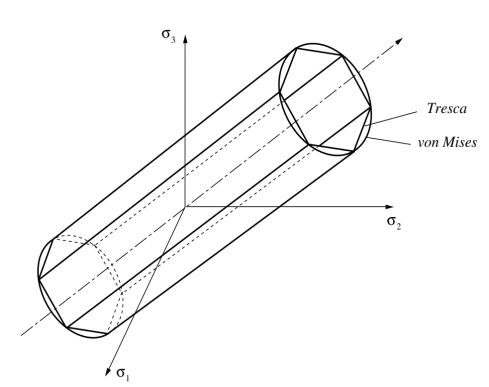
\includegraphics[width=0.7\linewidth]{images/Sup_trescaemises.png} % Do EA de souza Neto
    \label{fig:suptrescaemises}
    \fonte{\cite{neto_peric_owens_2008}}
\end{figure}

Outro critério muito conhecido é o de Tresca. Seu autor assume que a função que descreve a superfície de escoamento depende tanto de $ J_2 $ quanto de $ J_3 $. O terceiro invariante do tensor de tensões desviadoras, $ J_3 $, tem relação com a coordenada $ \theta $ de Haigh-Westergaard. Portanto, o estado de triaxialidade da tensão tem influência sob o escoamento neste critério. Em um plano desviador a superfície de escoamento de Tresca forma um hexaedro, vide figura \ref{fig:suptrescamises}, que coincide com a superfície de von-mises nos meridianos onde o ângulo $ \theta $ é múltiplo de $ 60º $. A menor distância entre o eixo hidrostático e a superfície de escoamento, no critério de Tresca, acontece nos ângulos múltiplos de $ 30º $ que significam estados de cisalhamento puro. A figura \ref{fig:trescamises} mostra a intersecção das superfícies de tresca e von Mises com um plano desviador qualquer.


\begin{figure}[H]
    \centering
    \caption{Projeção das superfícies de tresca e von Mises em um plano desviador.}
    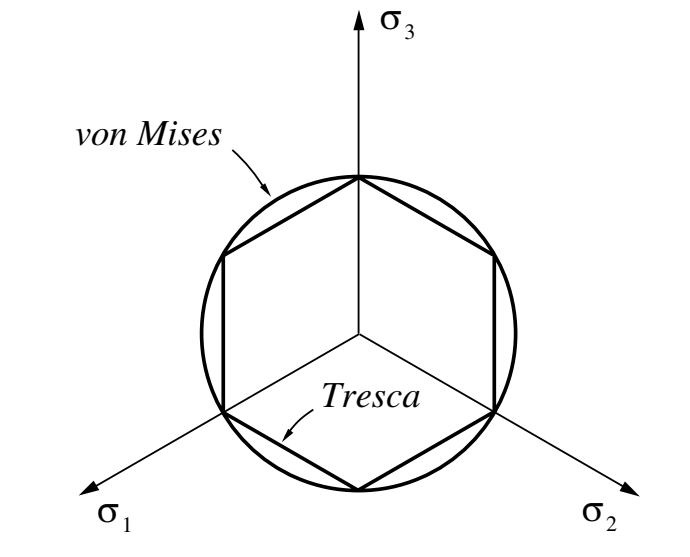
\includegraphics[width=0.7\linewidth]{images/trescaemises.png} % Do EA de souza Neto
    \label{fig:trescamises}
    \fonte{\cite{neto_peric_owens_2008}}
\end{figure}


\subsection{Escoamento dependente da pressão}

Apesar da pressão não influenciar o escoamento de materiais metálicos, ela deve ser levada em consideração quando outros materiais são simulados. Os critérios mais utilizados neste caso podem ser vistos como generalizações dos de Von-mises e de Tresca. A figura \ref{fig:mohrDrucker} mostra o critério de Mohr-Coulomb, que pode ser visto como uma generalização do critério de Tresca, e de Drucker-Prager, que generaliza o critério de Von-Mises.

\begin{figure}
    \centering
    \caption{Superfície de escoamento descrita pelos critérios de Mohr-Coulomb e Drucker-Prager}
    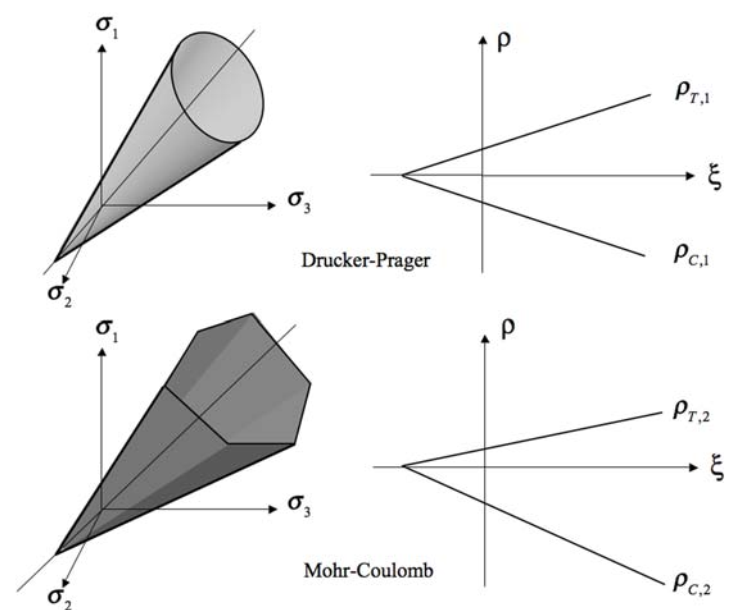
\includegraphics[width=0.7\linewidth]{images/tmohrdrucker.png}
    \label{fig:mohrDrucker}
     \fonte{\cite{neto_peric_owens_2008}}
\end{figure}

Tanto o critério de Mohr-Coulomb quanto o critério de Tresca apresentam descontinuidades na superfície de escoamento quando $\theta$ é multiplo de $ 60º $. Fato que, de acordo com  \cite{hiermaier_2008}, gera complicações numéricas quando algoritmos de retorno são usados para calcular a deformação plástica. Estes são os algorítmos mais usados quando um impacto balístico é simulado, sendo assim é apresentado um terceiro critério de falha na figura \ref{fig:Willamwarnke}, que é o de Willam-Warnke. A superfície descrita é suave para todos os ângulos $\theta$ facilitanto a aplicação de algoritmos de retorno. 

\begin{figure}
    \centering
    \caption{Superfície de escoamento descrita pelo critério de Willam-Warnke}
    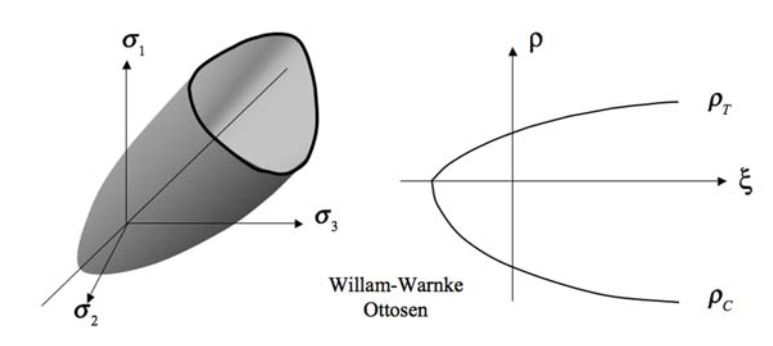
\includegraphics[width=0.7\linewidth]{images/willianwarnke.png} 
    \label{fig:Willamwarnke}
     \fonte{\cite{neto_peric_owens_2008}}
\end{figure}

\section{As funções de escoamento}

De acordo com \cite{neto_peric_owens_2008} a função de escoamento é responsável por aplicar o critério de escoamento usado. Inicialmente é imposto que a deformação plástica pode ocorrer apenas quando a função de escoamento $ \phi $ é nula.

\begin{equation}
     \phi(\boldsymbol{\sigma}, \boldsymbol{A}) = 0 
\end{equation}

Onde \gls{Cauchy} é o tensor de tensão de Cauchy, e $\boldsymbol{A}$ é um conjunto de variáveis termodinâmicas que estão ligadas ao encruamento.\\

De acordo com \cite{neto_peric_owens_2008} o seguinte conjunto, chamado domínio elástico é definido. 

\begin{equation}
    \mathcal{E} = \{ \gls{Cauchy} | \phi(\boldsymbol{\sigma}, \boldsymbol{A}) < 0   \}
\end{equation}

Em todo este conjunto as deformações plásticas não são permitidas. A visualização deste conjunto é auxiliada pelo espaço de tensões principais. Neste espaço o conjunto é formado pelos pontos onde a coordenada $\rho$ é menor do que a da superfície de escoamento. Note que a função de escoamento não restringe o tensor de tensões ao espaço principal, este é apenas um auxilio para o entendimento. As funções de escoamento são escritas levando em consideração o tensor descrito de forma geral, assim como a superfície de escoamento em seis dimensões.\\

O escoamento só pode ocorrer quando a tensão se localiza na superfície de escoamento, portanto esta é atingida quando a tensão faz parte do seguinte conjunto

\begin{equation}
    \mathcal{Y} = \{ \gls{Cauchy} | \phi(\boldsymbol{\sigma}, \boldsymbol{A}) = 0   \}
\end{equation}


\cite{neto_peric_owens_2008} apresenta a união destes dois conjuntos. Esta união forma um novo conjunto, chamado de tensões plasticamente admissíveis ou simplesmente tensões admissíveis.

\begin{equation}
    \overline{\mathcal{E}} = \{ \gls{Cauchy} | \phi(\boldsymbol{\sigma}, \boldsymbol{A}) \leq 0   \}
\end{equation}

No conjunto de tensões admissíveis estão todas as tensões que o material pode assumir em qualquer momento. Sendo assim, tensões com coordenada $\rho$ superiores à da tensão de escoamento são inadmissíveis. \par

Além da função de escoamento é necessário definir uma expressão para o fluxo do material quando este está deformando plasticamente. A lei de fluxo é responsável tanto pela taxa de deformação quanto por sua direção.

\begin{equation}
    \dot{\varepsilon}^p = \dot{\gamma} \boldsymbol{N}
\end{equation}

Onde \gls{gamma} é chamado de multiplicador plástico, ele define a magnitude da taxa de variação da deformação plástica.  \gls{N} é o vetor fluxo plástico. Este é um vetor é unitário, normal à superfície de escoamento e é definido da seguinte forma

\begin{equation}
    \boldsymbol{N} = \frac{\partial \boldsymbol{\Psi}}{\partial \boldsymbol{\sigma}} = \frac{\partial \boldsymbol{\phi}}{\partial \boldsymbol{\sigma}}
\end{equation}

Onde $\boldsymbol{\Psi} = \boldsymbol{\Psi}(\boldsymbol{\sigma}, \boldsymbol{A}) $ é o chamado potencial de fluxo. Porém assume-se, neste trabalho, que todos os modelos são associativos, portanto $ \boldsymbol{\Psi} = \boldsymbol{\phi} $. O vetor de Prandt-Reuss é o vetor de fluxo plástico aplicado à superfície de von-mises. No espaço das tensões principais ele tem direção normal ao círculo formado pela superfície em um plano desviador.

\section{As funções de encruamento}

As funções de encruamento são responsáveis por relacionar a tensão de escoamento às variáveis de estado relevantes. Alguns exemplos de variáveis de estado que podem ser consideradas são: A deformação plástica acumulada $ \overline{\varepsilon}^p $, a taxa de deformação $ \dot{\varepsilon} $ e a temperatura $ T $. A escolha das variáveis envolvidas depende do uso pretendido e da abordagem de um determinado grupo de pesquisa. Existem tanto modelos micromecânicos que levam em consideração a estrutura do , quanto modelos fenomenológicos que levam apenas a resposta macroscópica em consideração. Para apresentar funções de encruamento é interessante que se tenha em vista a função de escoamento na qual o encruamento é aplicado, dado que a tarefa da função de encruamento é alterar as características da superfície de escoamento. A formulação de von-mises será usada para apresentar as funções de encruamento pertinentes ao âmbito de impacto balístico já que ela é simples e de fato é base para muitos modelos. \\

A função de escoamento de von-mises assume que a deformação plástica ocorre quando o invariante $ J_2 $ assume um valor crítico.
\begin{equation} \label{eq:vonesc}
    \boldsymbol{\phi}(\boldsymbol{\sigma}) = \sqrt{J_2} - \tau_y
\end{equation}

Onde $ \tau_y $ é a tensão de escoamento inicial em cisalhamento. Ela se relaciona com a tensão de escoamento em tração uniaxial da seguinte forma.
\begin{equation}
    \sigma_y = \sqrt{3}\tau_y
\end{equation}

De acordo com \cite{neto_peric_owens_2008} usando esta relação e sabendo que 
$ J_2 = \frac{1}{3}\boldsymbol{\sigma}^2 $
é possível escrever a função de escoamento de von-mises da seguinte forma,

\begin{equation} \label{eq:vonesc}
    \boldsymbol{\phi}(\boldsymbol{\sigma}) = q(\boldsymbol{\sigma}) - \sigma_y = \sqrt{3 J_2} - \sigma_y
\end{equation}

 A função  $ q(\sigma) $ é amplamente conhecida como tensão de von-mises ou tensão equivalente. Portanto, de acordo com a função de escoamento de Von-Mises o escoamento ocorre quando a tensão equivalente é igual à tensão de escoamento naquele ponto.
 
 \subsection{Modelo da plasticidade isotrópica ou cinemática}

De acordo com \cite{rao_narayanamurthy_simha_2016} a expressão da tensão de von mises em uma dimensão para este modelo é a seguinte 

\begin{equation}
    \sigma_y = \left[1 + (\frac{\dot{\varepsilon}}{C})^{(\frac{1}{P})} \right](\sigma_0 + \beta E^p \overline{\varepsilon}^p)
\end{equation}

Este é baseado nos modos clássicos de plasticidade citados anteriormente. Nele $ \beta $ é chamado de parâmetro de endurecimento. Quando $ \beta = 0 $ o encruamento é completamente cinemático, caso $ \beta = 1 $ é completamente isotrópico, sendo permitidos valores de $ \beta $ entre $0$ e $1$. $ E^p $ é o módulo tangente ou o coeficiente de encruamento plástico, de acordo com \cite{neto_peric_owens_2008} quando generalizado para três dimensões
este se torna um tensor de quarta ordem. Já $\gls{defplastacu}$ é a deformação plástica acumulada, que pode ser calculada de acordo com a equação \ref{eq:defplastacu}. $ \sigma_0 $ é a tensão de escoamento inicial, $\dot{\varepsilon} $ é a taxa de deformação. Finalmente $ C $ e $ P $ são parâmetros da taxa de deformação de Cowper-Symonds. \par 

\begin{equation} \label{eq:defplastacu}
    \overline{\varepsilon}^p = \int_0^t |\dot{\varepsilon}^p| dt
\end{equation}

De acordo com \cite{rao_narayanamurthy_simha_2016} este tipo de modelo é o mais simples em termos da obtenção dos parâmetros necessários para uma simulação de impacto balístico, já que é de origem estática. Ele é aplicável a situações onde a velocidade do impacto é baixa e os efeitos térmicos podem ser ignorados. \cite{rao_narayanamurthy_simha_2016} afirma também que este modelo serve para prever satisfatoriamente
 parâmetros como a velocidade residual, profundidade de penetração e padrões de deformação.
 
 %CONTINUAR REVISAO
 \subsection{Modelo de Johnson-Cook}
 
 O modelo de Johnson-Cook é um modelo empírico que data de 1983 e é o mais usado quando o comportamento de metais em regimes dinâmicos é simulado. Ele leva em consideração os efeitos tanto da taxa de deformação quanto da temperatura na tensão de escoamento. A expressão da tensão equivalente, em uma dimensão, para este modelo é a seguinte
 
 \begin{equation}
     \sigma_y = [A + B (\overline{\varepsilon}^p)^n][1 + C ln(\dot{\varepsilon}^*)][1-(T^*)^m]
\end{equation}
 na qual 
\begin{align}
     \dot{\varepsilon}^* = \frac{\dot{\overline{\varepsilon}}^p}{\dot{\varepsilon}} &&
     T^* = \frac{T-T_r}{T_m-T_r}
 \end{align}
 
 $A$ é a tensão inicial de escoamento, $ B $ é o coeficiente de encruamento e $ n $ é o expoente de encruamento, $ \overline{\varepsilon}^p $ é a deformação plástica acumulada,  $\dot{ \overline{\varepsilon}^p} $  é a taxa da deformação plástica acumulada, $ \dot{\varepsilon}_0 $ é a taxa de deformação de referência e C é o coeficiente da taxa de deformação. Veja que $ T_m $ é a temperatura de fusão e $ T_r $ 
é a temperatura de referência, normalmente $ 298 \, K $ e $ m $ é o expoente térmico. \\

O primeiro termo entre colchetes relaciona a resistência dinâmica do material com o encruamento. De acordo com \cite{Crouch} o encruamento é o aumento da resistência do material devido a interação de discordâncias entre si e com barreiras externas. O empilhamento de discordâncias no contorno de grão ou em fases secundárias gera uma tensão contrária à aplicada e acaba aumentando a 
resistência do material à deformação. \\

O segundo termo entre colchetes é relacionado com a sensibilidade da resistência do material a diferentes taxas de deformação. \cite{Crouch} cita uma série de estudos que evidenciam a sensibilidade dos metais à taxa de deformação. Na fig \ref{fig:taxadef} é apresentado o efeito da taxa de deformação em alguns deles.

\begin{figure}[H]
    \centering
    \caption{Efeito da taxa de deformação na tensão de escoamento e na tensão máxima suportada de alguns aços.}
    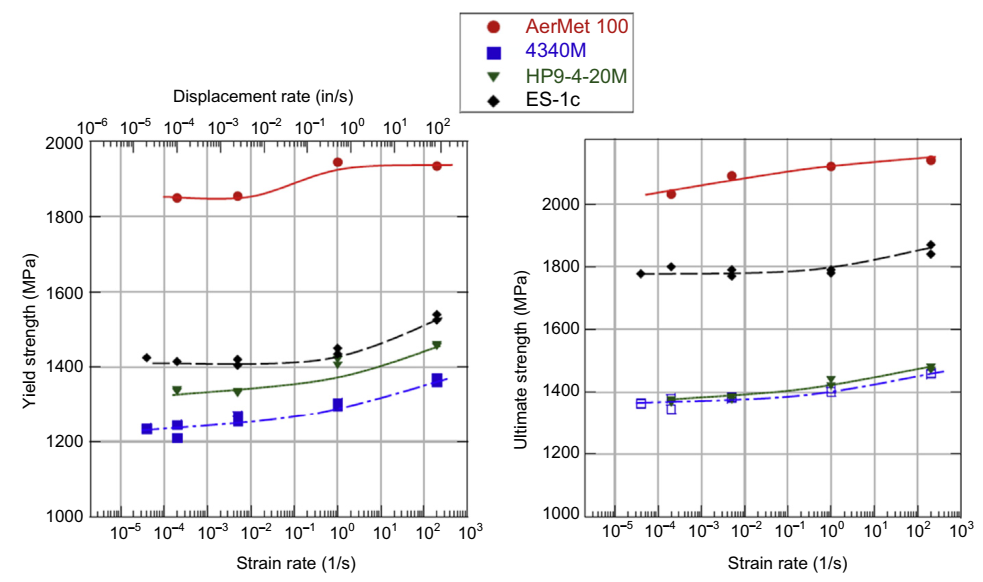
\includegraphics[width=0.5\linewidth]{images/strainrateeffect.png} 
    \label{fig:taxadef}
    \fonte{\cite{Crouch}}
\end{figure}

O terceiro termo tem relação com a temperatura, portanto ele diz respeito a diminuição da resistência do material devida ao aumento da temperatura. De acordo com \cite{Crouch} assume-se que o acréscimo de temperatura ocorre de forma adiabática e a fórmula para o cálculo do aumento da temperatura é a que segue

\begin{equation}
    \Delta T = \int_0^{\overline{\varepsilon}} \mathcal{X} \frac{\sigma_{eq}}{\rho C_p} d\overline{\varepsilon}
\end{equation}

Aqui o símbolo $ \mathcal{X}$ é novamente utilizado porém com outro sentido, algo não recomendado mas necessário para manter a identificação dos símbolos encontrados em diferentes literaturas. Neste caso $ \mathcal{X} $ é o coeficiente de Taylor-Quinney que em geral é 0.9.\footnote{Antes o símbolo $\mathcal{X}$ significava a função movimento, no contexto da cinemática.} $C_p$ é o calor específico do material, $ \rho $ a densidade, $ \sigma $ a tensão equivalente de von-mises e $ \varepsilon$ a deformação. 

\subsection{Modelo de dano de Johnson-Cook}

O modelo de dano de Johnson-Cook não é uma lei de encruamento, porém sua inserção neste tópico foi julgada adequada por conta de sua relação com o modelo de mesmo nome.
Este modelo de dano, também chamado critério de dano de Johnson-Cook, insere uma nova variável de estado chamada Dano. O dano no material varia de $ 0 $ a $ 1 $. A expressão usada para calcular o dano por este critério é a que segue

\begin{equation} \label{eq:danoincrJC}
    D = \sum \frac{\Delta \overline{\varepsilon}^p}{\varepsilon_f}
\end{equation}

Sendo $ \overline{\varepsilon}^p $ novamente a deformação plástica acumulada e $ \varepsilon_f $ a deformação de falha, calculada da seguinte forma

\begin{equation}
    \varepsilon_f = (D_1 + D_2 exp(D_3 \sigma^*))(1 + D_4 ln(\dot{\varepsilon}^*))(1 + D_5 T^*)
\end{equation}

De acordo com \cite{Crouch} o primeiro termo entre parenteses tem relação com a triaxialidade da tensão, o segundo toma conta do decréscimo da deformação de falha com o aumento da taxa de deformação e o terceiro relaciona o aumento da deformação de falha com o aumento da temperatura. \\

A expressão \ref{eq:danoincrJC} é a mais utilizada na literatura, porém está descrita de forma incremental. Esta é a forma usada para a implementação computacional dos modelos, mas ela não será abordada neste trabalho. A forma continua da mesma expressão é a que segue.

\begin{equation}
    D = \frac{\overline{\varepsilon}^p}{\varepsilon_f}
\end{equation}

Na qual a deformação plástica acumulada é calculada de acordo com \ref{eq:defplastacu}.

O critério de dano de Johnson-Cook é o mais usado para metais e normalmente a função de encruamento que leva o mesmo nome é complementada por este critério. Apesar disto nada impede o acoplamento deste critério com outras funções de encruamento. A consequência da falha no material pode ser lida de diversas formas e normalmente os códigos de propagação de onda apresentam opções para diferentes abordagens. Um elemento que falhou completamente, ou seja com $ D = 1  $, pode ser tanto retirado da simulação, por meio do mecanismo de erosão, quanto mantido suportando apenas tensões compressivas. Um dos usos para o dano é a redução da resistência ao escoamento, neste caso ele é tratado como uma variável interna.

\subsection{Modelo de Zerilli-Armstrong}
 
 Este modelo, diferente do modelo de Johnson-Cook, leva em consideração a estrutura cristalina do material. Ele existe em duas versões. A primeira é válida para materiais que assumem a estrutura cúbica de face centrada, CFC, e segue a expressão \ref{eq:ZA1}. A segunda vale para materiais constituídos pela estrutura cubica de corpo centrado, CCC, que é apresentada em \ref{eq:ZA2}. \\
 
 \begin{equation} \label{eq:ZA1}
     \sigma_y = C_0 + C_1 exp[-C_3T + C_4Tln(\dot{\overline{\varepsilon}}^p)] + C_5 (\overline{\varepsilon}^p)^n
 \end{equation}
 
  \begin{equation} \label{eq:ZA2}
     \sigma_y = C_0 + C_2\sqrt{\overline{\varepsilon}^p}exp[-C_3T + C_4Tln(\dot{\varepsilon}^p)] 
 \end{equation}
 
Onde $C_0$,$C_1$,$C_2$,$C_3$,$C_4$ são parâmetros de ajuste, $ C_5 $ é o coeficiente de encruamento e n é o expoente de encruamento. \\

O que motiva a apresentação de modelos diferentes de acordo com a estrutura cristalina dos metais é a diferença entre os mecanismos que coordenam a deformação plástica para diferentes estruturas cristalinas.
 
 \subsection{Modelos de Johnson-Holmquist}
 
 Os modelos de Johnson-Holmquist são os mais usados para simular o comportamento de cerâmicos durante um impacto em alta velocidade. Existem três versões deste modelo, porém as mais usadas são a primeira e a segunda. A terceira versão não será apresentada, ela é uma relaeitura da primeira versão. O primeiro modelo de Johnson-Holmquist é também chamado de JH-1, consequentemente o segundo é o JH-2.  \\
 
 Todos os três modelos descrevem a tensão equivalente como dependente da pressão. Uma interpretação possível é que a superfície de escoamento para estes modelos se assemelha com a de Drucker-Prager, porém para afirmar categoricamente como de fato é a superfície é necessário ter acesso à implementação dos modelos. O relatório \cite{JH2Imp} fala sobre a implemetação do segundo modelo de Johnson-Holmquist,
 porém trata $ \dot{\varepsilon}^p $ como um valor já disponível. Como dito anteriormente este valor é dependente de um mutiplicador e de um vetor de fluxo plástico, sendo assim ele não está naturalmente disponível e deve ser calculado. Duas são as possibilidades para o motivo de assumir este valor como dado. \\
 
 A primeira possibilidade é assumir que como o autor do relatório usa nomes compatíveis com a teoria de von-miese, ele chama a tensão de equivalente e a deformação de equivalente, subentende-se que o critério de von-mises é usado e portanto não seria errado inferir que o vetor de fluxo é o de Prandt-Reuss. Sendo assim o autor do relatório não quis se prolongar em tal discussão e tomou a informação como dada. \\
 
 A possibilidade alternativa 
 é que a implementação deste vetor possa estar protegida por um segredo industrial e fica de fato dúbio qual vetor de fluxo é usado. Esta dificuldade se repete para todos os modelos de Johnson-Holmquist, ao menos na porção da literatura pesquisada. A segunda possibilidade é corroborada por uma discussão no site acadêmico Researchgate.\footnote{ O sitio onde está a pergunta e posterior discussão é  \url{https://www.researchgate.net/post/How_can_I_implement_JH-2Johnson_holmquist_constitutive_equation_in_explicit_FEM} } Nesta um pesquisador solicita ajuda para implementar o segundo modelo de Johnson-Holmquist pois não consegue calcular corretamente $ \dot{\varepsilon}^p $ gerando erros em seus resultados. Julgando que a falta desta informação não prejudica a simples apresentações dos modelos que aqui será feita. O primeiro modelo de Johnson-Holmquist é apresentado a seguir. \\
 
 \subsubsection{O primeiro modelo de Johnson-Holmquist}
 
O primeiro modelo de de Johnson-Holmquist usa uma descrição polinomial por partes da tensão equivalente. De acordo com \cite{holmquist_johnson_2002} a resistência inicial do material intacto $ \sigma_0 $ é representada por uma função formada por segmentos de reta que é ajustada de acordo com o material. Esta função é representada pela linha contínua superior da figura \ref{fig:JH1Tensao}. Esta resistência é relacionada a uma taxa de deformação adimensional
\begin{equation}
    \dot{\varepsilon}^* = \dot{\varepsilon}/\dot{\varepsilon_0}
\end{equation}
onde $ \dot{\varepsilon_0} $ 
é a taxa de deformação de referência e é normalmente equivalente a $1.0 s^{-1} $. Quando $ \dot{\varepsilon}^* = 1.0 $ a resistência do material é $ \sigma_0 $. Para taxas diferentes de deformação adimensional é aplicada expressão \ref{eq:JH1tensao}, onde $ C $ é chamada constante da taxa de deformação e tem relação com a sensibilidade do material à velocidade de solicitação. 

\begin{equation} \label{eq:JH1tensao}
    \sigma_y = \sigma_0(1.0 + C ln\dot{\varepsilon}^*)  
\end{equation}

\begin{figure}[H] 
    \centering
    \caption{Relação entre a tensão de von-mises e a Pressão para o primeiro modelo de Johnson-Holmquist}
    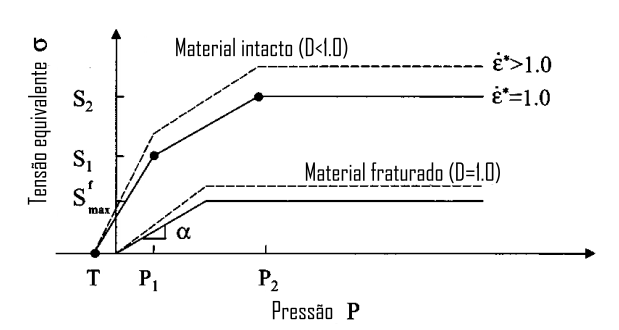
\includegraphics[width = 0.7\linewidth]{images/sigmapressao.png} 
    \label{fig:JH1Tensao}
    \fonte{\cite{holmquist_johnson_2002}}
\end{figure}


A expressão \ref{eq:JH1tensao} é responsável por descrever a resistência do material intacto, por intacto entende-se que o dano $ D \neq 1 $. Diferente de todos os modelos vistos até agora a resistência do material depende do dano, assim há outra curva que descreve a resistência do material que falhou. O modelo de dano é acoplado à função de encruamento, consequntemente é apresentado a seguir. 
O dano é calculado de forma semelhante ao de Johnson-Cook. O cálculo é novamente apresentado da forma incremental. 

\begin{equation} \label{eq:danoJH}
    D = \sum \frac{\Delta \overline{\varepsilon^p} }{\varepsilon^p_f}
\end{equation}

A Diferença entre as duas é o termo $ \varepsilon^p_f $ que é chamado deformação de falha e é calculado através da seguinte expressão

\begin{equation}
    \varepsilon^p_f = \phi(P_3 + T)
\end{equation}

Onde $ P_3 $ é a pressão em que ocorre a saturação da deformação de falha, que pode ser vista na figura \ref{fig:deffalhapressJH1}. $ T $ é a tensão hidrostática trativa máxima, na qual a deformação de falha é nula e quando atingida o material falha instantaneamente. Esta tensão está representada na figura \ref{fig:JH1Tensao} pela letra $T$. $ \phi $ é o coeficiente angular da reta descrita pela deformação de falha antes da saturação, calculado da seguinte maneira

\begin{equation}
    \phi = \ddfrac{\varepsilon^{max}_{f}}{(P_3 + T)}
\end{equation}

\begin{figure}
    \centering  
    \caption{Relação da deformação de falha com a pressão}
    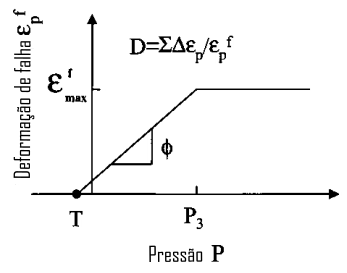
\includegraphics[width = 0.7\linewidth]{images/deffalhapressao.png} 
    \label{fig:deffalhapressJH1}
    \fonte{\cite{holmquist_johnson_2002}}
\end{figure}

Na figura \ref{fig:JH1Tensao} também está presente a descrição da resistência do material que atingiu a condição de falha, ou seja $ D = 1 $. Esta resistência é descrita usando dois parâmetros do modelo, que são particularmente difíceis de se obter usando experimentação. Devido a dificuldade de obtenção experimental, a definição destes é feita através da calibração da simulação de um teste balístico. \cite{holmquist_johnson_2002} aponta que tal característica do modelo não é desejável, porém a simulação do material sem estes dois patamares de força leva a resultados insatisfatórios.
Os parâmetros citados são $ \alpha $ que é o coeficiente angular da reta que representa a resistência do material que falhou até atingir $ S^{max}_f $, que é a resistência máxima do material falhado. \par

Este modelo apresenta outra particularidade, que é o acoplamento de uma  equação de estado. A pressão no material é caracterizada pela seguinte expressão 

\begin{equation} \label{eq:JHEOS}
    P = K_1 \mu + K_2 \mu^2 + K_3 \mu^3
\end{equation}

\begin{figure} \label{fig:pressvsdefvolJH1}
    \centering
    \caption{Relação entre a pressão e a deformação volumétrica} 
    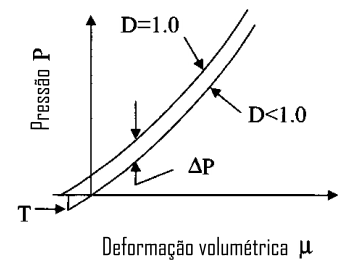
\includegraphics[width=0.7\linewidth]{images/defvolpressao.png}
    \label{fig:my_label}
    \fonte{\cite{holmquist_johnson_2002}}
\end{figure}

Na qual $ \mu $ representa a deformação volumétrica do corpo e é calculada da seguinte maneira

\begin{equation}
    \mu = \frac{V_r}{V} - 1 = \frac{\rho}{\rho_r} - 1
\end{equation}

Onde $ K_1 $, $ K_2 $ e $ K_3 $ são constantes. $ K_1 $ é o módulo volumétrico do material, já as outras não tem leitura física definida. Para pressões negativas, ou tensões hidrostáticas trativas, a expressão  \ref{eq:JHEOS} é substituída por $ P = K_1 \mu $. \\


De acordo com \cite{holmquist_johnson_2002}
quando o material falha o modelo permite que haja um acréscimo $ \Delta P $ na pressão, de forma que 

\begin{equation} \label{eq:EOSJH2}
	P = K_1 \mu + K_2 \mu^2 + K_3 \mu^3 + \Delta P
\end{equation}


Este acréscimo de pressão é decorrente da redução da energia elástica interna  do material que se deve ao decréscimo das tensões desviadoras no local. A expressão da energia elástica interna no material é a seguinte

\begin{equation}
	e_{el} = \ddfrac{\sigma_{eq}^2}{6G}
\end{equation}

Na qual $ G $ é o módulo de cisalhamento. \\

Novamente de acordo com \cite{holmquist_johnson_2002}

a  energia elástica perdida pode ser transformada em energia potencial hidrostática, que se apresenta no termo adicional $ \Delta P $ da expressão \ref{eq:EOSJH2}. A expressão para calcular $\Delta P$ é a seguinte

\begin{equation} \label{eq:JHEOSDeltaP}
	\Delta P = -K_1 \mu_f + \sqrt{(K_1 \mu_f)^2 + 2 \beta K_1 \Delta e_{el}}
\end{equation} 

Onde $ \mu_f $ é a deformação volumétrica no momento da falha. O termo $ \beta $ é uma constante do material, de forma que se $ \beta = 0 $, então $ \Delta P = 0 $ e nenhuma energia elástica interna é transformada em potencial hidrostática. Se $ \beta = 1 $ toda energia elástica perdida é alocada e $ \Delta P $ tem seu valor máximo. \\


As figuras \ref{fig:JH1Tensao}, \ref{fig:deffalhapressJH1} e \ref{fig:pressvsdefvolJH1} são bons resumos do primeiro modelo de Johnson-Holmquist. Mesmo se tratando do primeiro modelo ele ainda é muito usado por obter bons resultados e ser simples. Uma característica importante dele é que não permite redução da resistência do material com o aumento do dano, o que ocorre é uma redução abrupta quando o dano atinge o valor crítico $ D = 1 $. Por conta disto este modelo é usado nos materiais que apresentam tal caracterísica como por exemplo o carbeto de silício. Defirente do JH-1 o modelo JH-2 apresentado a seguir permite que a resistência do material diminua ao longo do processo de danificação. \par

\subsubsection{O segundo modelo de Johnson-Holmquist}

Como foi dito anteriormente o segundo modelo de Johnson-Holmquist permite a redução da resistência do material a medida que este é danificado, este comportamento pode ser visto na figura \ref{fig:JH2tensao}. Este modelo usa uma normalização de seus parâmetros que usa dados do limite elástico de Hugoniot. O limite elástico de Hugoniot será explicado no próximo capítulo mas é basicamente a tensão a partir da qual o material começa a se deformar plasticamente em um ensaio uniaxial de deformação.

As tensões neste modelo são todas normalizadas da seguinte forma $ \sigma^* = \sigma/\sigma_{LEH} $ onde $ \sigma_{LEH} $ é a tensão no limite elástico de Hugoniot ou LEH. $ \sigma $ é a tensão equivalente, que segue a seguinte expressão

\begin{equation} \label{eq:JH2tensao}
    \sigma^* = \sigma^*_i - D(\sigma^*_i - \sigma^*_f)
\end{equation}

Na qual $ \sigma^*_i $ é a resistência inicial normalizada e $ \sigma^*_f $ é a resistência normalizada do material fraturado. Estas duas podem ser respectivamente calculadas de acordo com as expressões \ref{eq:tensaoinicialJH2} e \ref{eq:tensaofraturadaJH2}.

\begin{equation} \label{eq:tensaoinicialJH2}
    \sigma^*_i = A(P^* + T^*)^N (1 + C ln\dot{\varepsilon}^*)
\end{equation}

\begin{equation}
    \sigma^*_f = B(P^*)^M(1 + Cln\dot{\varepsilon}^*)
\end{equation}

Nas quais $A$, $B$, $C$, $M$ e $N$ são constantes do material. Em  \cite{johnson_holmquist_1994} o autor do modelo cita que é possível limitar $ \sigma^*_f $, de modo que este fique menor ou igual a $ S^{max}_f $ que novamente é a resistência máxima do material pós falha. O autor não fala nada sobre a tensão pós falha ser ou não normalizada, mas levando em consideração que o modelo é todo normalizado seria prudente usar $ (S^{max}_f)^*$. 
A taxa de deformação normalizada $ \dot{\varepsilon}^* $ tem o mesmo significado e é calculada da mesma forma que no primeiro modelo. $ P^* $ é a pressão normalizada, sendo \begin{equation}
    P^* = P/ P_{LEH} 
\end{equation}  

$ T^* $ é a tensão hidrostática trativa máxima normalizada, calculada da seguinte maneira \begin{equation}
    T^* = T/P_{LEH} 
\end{equation}   
\begin{figure}
    \centering
    \caption{Tensão equivalente normalizada no segundo modelo de Johnson-Holmquist}
    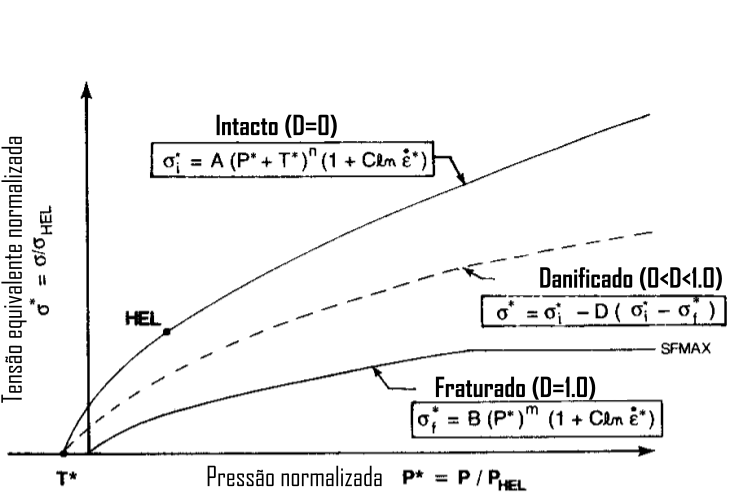
\includegraphics[width=0.7\linewidth]{images/sigmapressaoJH2.png}
    \label{fig:JH2tensao}
    \fonte{\cite{johnson_holmquist_1994} traduzida pelo autor.}
\end{figure}

O segundo modelo de Johnson-Holmquist calcula o dano seguindo a expressão \ref{eq:danoJH}, que é a mesma do primeiro modelo, porém a deformação de falha $ \varepsilon^p_f $ agora é calculada da seguinte maneira

\begin{equation}
    \varepsilon^p_f = D_1(P^* + T^*)D^2
\end{equation}

Onde $ D_1 $ e $ D_2 $ são constantes do material % TODO: Verificar como estas CTES são calculadas, se n é por calibração
e novamente quando a tensão hidrostática ou pressão no material é trativa e igual a $ -T^* $ o material não é capaz de suportar qualquer deformação e falha de forma instantânea. O comportamento da deformação de falha é apresentado na figura \ref{fig:danoJH2}.

\begin{figure}
    \centering
    \caption{Comportamento da deformação de falha equivalente.}
    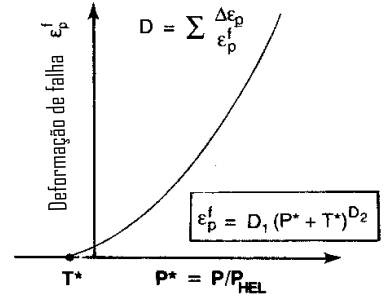
\includegraphics[width=0.7\linewidth]{images/deffalhaJH2.png} 
    \label{fig:danoJH2}
    \fonte{\cite{johnson_holmquist_1994} traduzida pelo autor.}
\end{figure}

Novamente o modelo apresenta uma equação de estado acoplada, que segue a expressão \ref{eq:JHEOS}. Neste caso o acréscimo da pressão acontece de forma gradual, já que o material vai perdendo resistência ao longo do processo de danificação. A expressão corrigida é idêntica, vide eq. \ref{eq:EOSJH2}. O autor apresenta $ \Delta P $ de forma incremental no artigo de apresentação do modelo, \cite{johnson_holmquist_1994} . Porém como a formulação incremental não será abordada, a equação \ref{eq:JHEOSDeltaP} permanece válida e pequenas parcelas de energia são transformadas em cada ciclo. 


 
 
 
 
 
 
 
 
 






